\section{Giới thiệu sản phẩm}
Bài tập lớn của chúng em mô phỏng hai khung cảnh chính sau:
\begin{itemize}
    \item Khung cảnh ngoài trời
    \item Khung cảnh trong ngôi nhà 
\end{itemize}
\subsection{Khung cảnh ngoài trời}
Trong phần này, chúng em mô phỏng khung cảnh một ngôi nhà nằm giữa rừng cây và thêm hiệu ứng những đám mây đang trôi trên bầu trời. Khung cảnh được hiện lên trong hai thời điểm: ban ngày và ban đêm. 
\begin{center}
    \begin{figure}[!h]
        \centering
        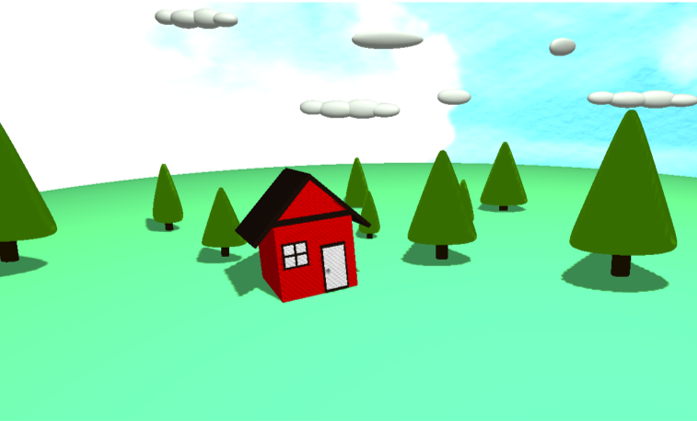
\includegraphics[scale = 0.85]{contents/out day.png}
        \caption{Khung cảnh ngoài trời vào ban ngày}
    \end{figure}
\end{center}
\newpage 
\begin{center}
    \begin{figure}[!h]
        \centering
        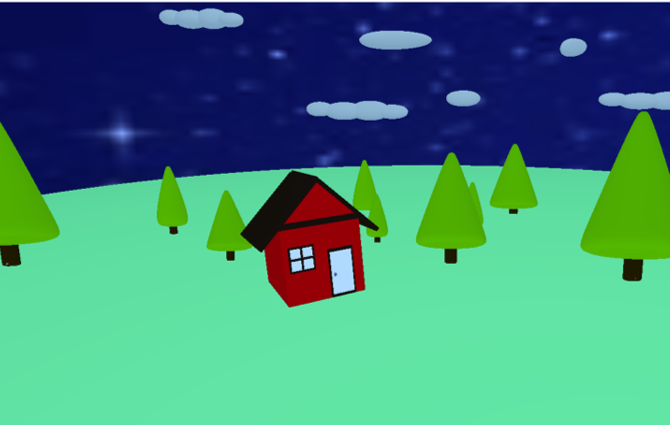
\includegraphics[scale = 0.85]{contents/outdoornight.png}
        \caption{Khung cảnh ngoài trời vào ban đêm}
    \end{figure}
\end{center}
\subsection{Khung cảnh trong ngôi nhà}
Trong phần này, chúng em mô phỏng khung cảnh bên trong ngôi nhà gồm các đối tượng: giường, tủ, bàn học, chậu cây, thảm,... Các đối tượng này được sắp xếp vào các vị trí phù hợp với nhau.
\begin{center}
    \begin{figure}[!h]
        \centering
        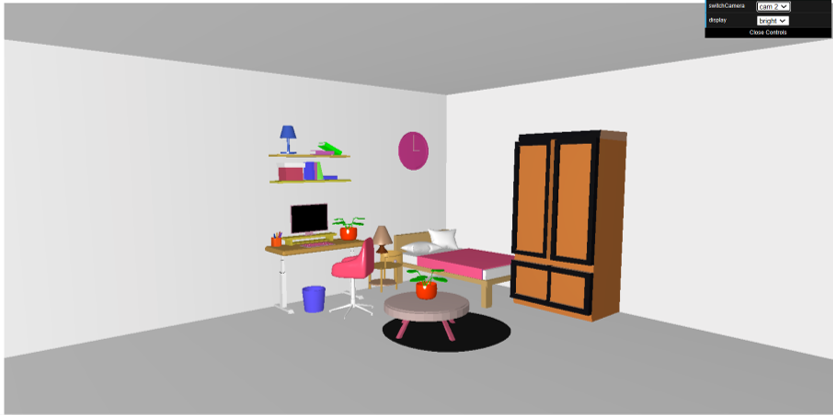
\includegraphics[scale = 0.7]{contents/trong nhà.png}
        \caption{Khung cảnh chi tiết trong nhà}
    \end{figure}
\end{center}
